\subsection{ViViT: A Video Vision Transformer}

\subsubsection{Overview}

\par Arnab \textit{et al}, in their 2021 paper titled \textit{ViViT: A Video Vision Transformer} \cite{vivit}, extend the Vision Transformer (ViT) \cite{vit} to tackle video recognition tasks. 
They propose various attention architectures to model the spatial and temporal interaction within video frames. 
The also propose embedding extraction methods for videos which are on similar lines to those done for images. \par

\subsubsection{Datasets}
\begin{itemize}
\item Pre-trained on:
	\begin{itemize}
		\item ILSVRC-2012 ImageNet dataset with 1k classes and 1.3M images
		\item ImageNet 21k dataset with 21k classes and 14M images 
		\item JFT with 18k classes and 303M high-resolution images
	\end{itemize}
\item Benchmark tasks
	\begin{itemize}
		\item Kinetics 400/600
		\item Epic Kitchens
		\item Something-Something v2
		\item Moments in Time
	\end{itemize}
\end{itemize}


\subsubsection{Performance}
\par Arnab \textit{et al} report state-of-the-art-performance for various video recognition tasks (datasets mentioned above), when compared with current SOTA models.\par


\subsubsection{Methodology}

\par Arnab \textit{et al} use the ViT model \cite{vit} as its foundation, but with different input embeddings that are extracted from video and different attention blocks. 
The transformer model then outputs a classification ([class]) token which represents the entire video. 
This [class] token is then used for downstream tasks (mentioned above).\par

\paragraph{Input: Token embeddings}

\par Two methods for mapping a video to its correspinding embeddings are proposed, namely:
\begin{itemize}
    \item \textit{Uniform frame sampling}
    \begin{itemize}
        \item The original video $x = R^{TxHxWxC}$.
        \item From this, we extarct $N = n_t.n_h.n_w$ tokens which are subsequently mapped to d-dimensional space. Here, $n_t$ corresponds to the number of frames in the video.
    \end{itemize} 
    \item \textit{Tubelet embedding}
    \begin{itemize}
        \item This method models the 3D convolutions or "tubes".
        \item $n_t = T/t$ frames are sampled, each with $n_h.n_w$ non-overlapping patches.
        \item From this, we extarct $N = n_t.n_h.n_w$ tokens which are subsequently mapped to d-dimensional space.

        \begin{figure}
            \centering
            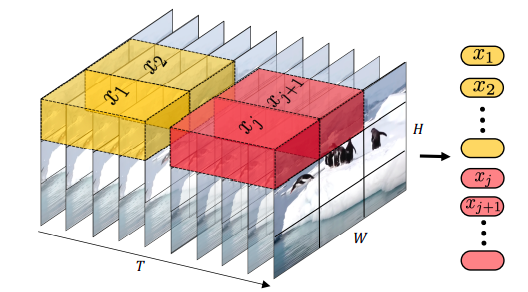
\includegraphics[width=\linewidth]{assets/img/vivit-tublet-embed.png}
            \caption{Video Transformer introduced by Arnab \textit{et al} (Courtesy \cite{vivit})}
        \end{figure}

    \end{itemize} 
    \item The final output consists of $x = R^{Nxd}$
    \item A learnable [class] token may be prepended to the token sequence based on the attention architecture being used.
\end{itemize}
\par

\paragraph{Transformer Encoder}

\par ViViT extends the transformer model proposed in \cite{vit} by making use of different attenion architectures to model the spatio-temporal interaction between the token embeddings. \par

\begin{figure}[h]
	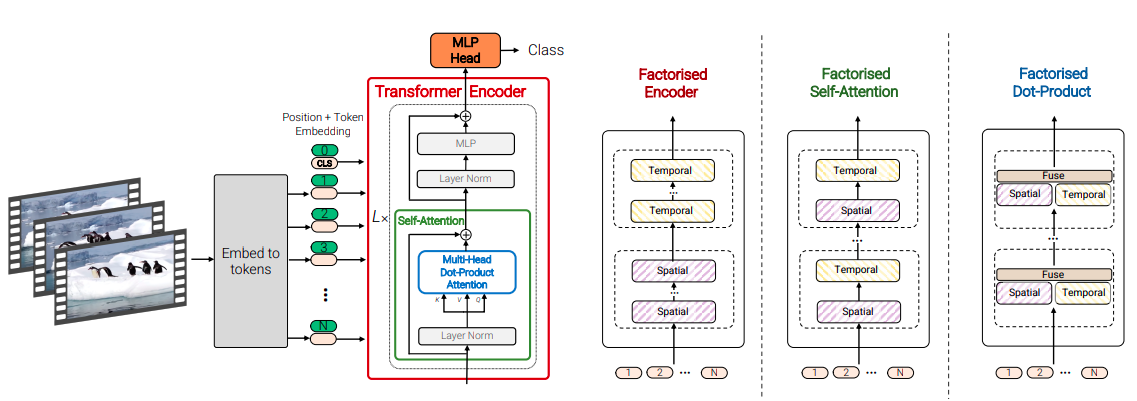
\includegraphics[width=\linewidth]{assets/img/vivit.png}
	\caption{Video Transformer introduced by Arnab \textit{et al} (Image courtesy \cite{vivit})}
\end{figure}

\par Four attention architectures are proposed, namely:
\begin{itemize}
    \item \textit{Spatio-temporal attention}
    \begin{itemize}
        \item This architecture mimics the multi-headed self attenion block \cite{tfm} across all ${Nxd}$ tokens.
        \item However, it has quadratic time complexity as it models all pairwise interactions between all spatio-temporal tokens.
    \end{itemize} 
    \item \textit{Factorised encoder}
    \begin{itemize}
        \item This architecture consists of two transformer encoders to model spatial and temporal interactions between the tokens separately.
        \item First, the spatial encoder gets $n_h.n_w$ tokens in order to attend to tokens within the same temporal index (same frame/tube).
        \item Next, $n_t$ [class] tokens representing $n_h.n_w$ tokens of each frame are given as input the the temporal encoder. 
        \item The temporal encoder outputs another [class] token which is the collective representation of all the frames in the video.
        \item Model 2 does have more parameters that model 1, but consists of fewer floating point operations due to a decrease in the number of tokens per encoder.
    \end{itemize}
    \item \textit{Factorised Self-Attention}
    \begin{itemize}
        \item This architecture consist of two multi-headed self attenion blocks within a single encoder.
        \item The first one models spatial interactions between tokens and the second one, temporal.
        \item The first attention block gets tokens $x = R^{n_txn_h.n_wxd}$ which include tokens within the same temporal index.
        \item The second attention block gets tokens $y = R^{n_h.n_wxn_txd}$ which include tokens within the same spatial index.
        \item Model 3 has fewer parameters but the same complexity as model 2.
    \end{itemize}
    \item \textit{Factorised Dot-Product Attention}
    \begin{itemize}
        \item This architecture aims to fuse the spatial and temporal attention within the same multi-headed self attenion block, but with different heads.
        \item The spatial attention heads get $x = R^{n_txn_h.n_wxd}$ tokens as input whereas the temporal attention heads get $y = R^{n_h.n_wxn_txd}$ as input.
        \item Model 4 has the same number of parameters as model 1 and the same complexity as models 2 and 3.
    \end{itemize}
    \item The final output can either be a [class] token or a 1D vector obtained by average pooling all output vectors.
\end{itemize}



\paragraph{Training Procedure}
\par Pre-trained weights of the ViT model are leveraged due to the size of various video recognition tasks (many orders of magnitude smaller than image recognition datasets).
The model can then be trained on various video recognition datasets such as Kinetics and Epic Kitchens.
\begin{itemize}
	\item Kinetics 
	\item Strong regularization is used throughout the encoder. Dropout, when used, is applied after every dense layer except for the the query-key-value projection layers and directly after the addition of positional embeddings
	\item Training is done on a resolution of 224 (14x14)
\end{itemize}

\subsubsection{Conclusion}
\par The work by Arnab \textit{et al} provides a compelling case for using transformers instead of CNN-architectures in video recognition tasks. 
Even though it requires large amount of pre-training, it can be scaled much better than its CNN counterparts and can meet the performance (and even exceed it in certain cases) of current SOTA CNN-based models.
